\documentclass[10pt, a4paper]{report}

\usepackage{listingsutf8}
\usepackage[utf8]{inputenc}
\usepackage[spanish]{babel}
\usepackage{amsfonts}
\usepackage{amsmath}
\usepackage{amssymb}
\usepackage{amsthm}
\usepackage{graphicx}
\usepackage{pdfpages}
\usepackage{spverbatim}
\usepackage{multirow}
\usepackage[left=3.5cm,right=1.5cm,top=2.5cm,bottom=2.5cm]{geometry}
\usepackage{xcolor}
\usepackage{textcomp}
\usepackage{listings}
\usepackage{hyperref}
\usepackage{floatrow}
\author{Daniel Fernández Villanueva}
\title{\huge Sistema de monitorización inercial del movimiento de las extremidades superiores}

\makeatletter
\renewcommand*{\UTFviii@defined}[1]{%
  \ifx#1\relax
    \begingroup
      % Remove prefix "\u8:"
      \def\x##1:{}%
      % Extract Unicode char from command name
      % (utf8.def does not support surrogates)
      \edef\x{\expandafter\x\string#1}%
      \StringEncodingConvert\x\x{utf8}{utf16be}% convert to UTF-16BE
      % Hexadecimal representation
      \EdefEscapeHex\x\x
      % Enhanced error message
      \PackageError{inputenc}{Unicode\space char\space \string#1\space
                              (U+\x)\MessageBreak
                              not\space set\space up\space
                              for\space use\space with\space LaTeX}\@eha
    \endgroup
  \else\expandafter
    #1%
  \fi
}
\makeatother

\setcounter{tocdepth}{3}
\usepackage{color}
\definecolor{dkgreen}{rgb}{0,0.6,0}
\definecolor{gray}{rgb}{0.5,0.5,0.5}
\definecolor{mauve}{rgb}{0.58,0,0.82}
\lstset{frame=tb,
  language=C++,
  aboveskip=3mm,
  belowskip=3mm,
  showstringspaces=false,
  columns=flexible,
  basicstyle={\small\ttfamily},
  numbers=left,
  frame=single,
  numberstyle=\tiny\color{gray},
  keywordstyle=\color{blue},
  commentstyle=\color{dkgreen},
  stringstyle=\color{mauve},
  breaklines=true,
  breakatwhitespace=true
  tabsize=4
}

\newtheorem{defn}{Definición}[section]

\begin{document}

\maketitle

\tableofcontents

\listoffigures

\listoftables

%%% ================ PARTE 1 : MEMORIA ================ %%%

\part{Memoria}

\pagestyle{headings}


%% ******** Capítulo 1 ******** %%

\chapter{ANTECEDENTES}


%% ******** Capítulo 2 ******** %%

\chapter{OBJETIVO DEL PROYECTO}

Este proyecto tiene como objetivo la implementación de un sistema de monitorización en tiempo real del movimiento de las extremidades superiores del cuerpo humano. Para la realización de este sistema se tendrá que dar solución a los siguientes

\begin{enumerate}
\item \textbf{Aplicación para la adquisición de datos de los sensores inerciales}: \\
Realización de un sistema que permitirá obtener en tiempo real los datos que proporcionan los sensores. En concreto se desarrollará un driver para un sensor xsens o una red de sensores xsens conectados mediante un master xbus. Este driver permitirá leer los datos que proporcionan los acelerómetros, giróscopos, magnetómetros y sensores de temperatura, además de la orientación de cada uno de los sensores conectados al PC. Este driver se encargará también de crear una interfaz para la posterior utilización de los datos en otros programas de foma sencilla. \\

\item \textbf{Tratamiento de los datos para obtener los ángulos de rotación entre cada sensor}:\\
Una vez sea posible la adquisición de los datos con el driver anterior, se creará otro programa con el que se obtendrán los ángulos de rotación entre cada sensor teniendo en cuenta además la geometría de las articulaciones del brazo o modelo sobre las que se situarán los sensores.\\

\item \textbf{Utilización de los datos para el objetivo deseado}: \\
En esta última fase se crearán los sistemas necesarios para la utilización de los datos con el objetivo deseado:

\begin{itemize}

\item Para la visualización de la posición del brazo en el simulador 3D Gazebo, se creará un modelo del brazo y una interfaz etre ROS y el simulador que permitirá la visualización de la posición del brazo en tiempo real.  

\item Para el control del robot mediante el movimiento del brazo o modelo del robot físico, se creará otra interfaz entre ROS y el driver del propio robot. 

\end{itemize}

\end{enumerate}


%%% ******** Capítulo 3 ******** %%%
\chapter{ESPECIFICACIONES DE DISEÑO}



%%% ******** Capítulo 4 ******** %%%
\chapter{DISEÑO DEL SISTEMA}

\section{Estudio de soluciones}
\section{Simulación}

%%% ******** Capítulo 3 ******** %%%
\chapter{IMPLEMENTACIÓN FÍSICA}
\section{Selección de componentes}
\section{Montaje}
\section{Ajuste}

\chapter{PROTOCOLO DE PRUEBAS. REDISEÑO}

\chapter{RESULTADOS OBTENIDOS}
%%% ******** Capítulo 5 ******** %%%
\chapter{HERRAMIENTAS UTILIZADAS}

En este capítulo se realizará una breve descripción de los elementos utilizados en el proyecto, tanto de hardware como de software.

\section{Hardware}

\subsection{Sensores XSENS}

\subsubsection{Sensor MTi-G}

\subsubsection{XBUS Master}

\subsection{Brazo humano}

\subsection{Robot Youbot}

\subsection{Modelo del robot Youbot}

\section{Software}

\subsection{ROS}

\subsubsection{¿Qué es ROS?}

ROS (del inglés \textit{Robot Operating System} - Sistema Operativo Robótico) es una plataforma de desarrollo de software que incluye conjunto de utilidades centradas en ayudar al desarrollador en la creación de programas para el control de robots. Esta herramienta incorpora abstracción del hardware, drivers para dispositivos, librerías, visualizadores, utilidades para el intercambio de mensajes entre programas y administradores de paquetes de software, entre otras muchas cosas. ROS es además software abierto, bajo una licencia BSD, por lo que cualquier persona puede ver su código fuente y modificarlo.

\subsubsection{¿Por qué usar ROS?}

ROS proporciona solución a diversos problemas que vienen dados inherentemente al objetivo de este proyecto:

\begin{itemize}

\item \textbf{Creación y compilación de programas}

\begin{itemize}

\item \textbf{Gestor de paquetes}

\end{itemize}

\item \textbf{Comunicación entre programas:}
ROS incluye:

\begin{itemize}

\item \textbf{Máster}

\item \textbf{Topics}

\item \textbf{Servicios}

\item \textbf{Servidor de parámetros}

\end{itemize}

\item \textbf{Visualización de datos}

\item \textbf{Otras herramientas}

\begin{itemize}

\item \textbf{Bag}

\item \textbf{rxplot}

\end{itemize}


\end{itemize}

\subsection{El sistema operativo Ubuntu}

\subsubsection{¿Qué es Ubuntu?}

Ubuntu es un sistema operativo con núcleo Linux. Es gratuito y es distribuido como software \textit{open source}. Se trata de la distribución GNU/Linux más popular en equipos personales

\subsubsection{¿Por qué usar Ubuntu?}

\subsection{El lenguaje de programación C++}



\subsection{Simulador Gazebo}

Gazebo es programa para simulación en 3D de un robot o una población de robots interactuando entre sí y el ambiente. Incorpora simulación de la física de sólidos rígidos y de la respuesta de sensores. Además incorpora un visualizador 3D bastante potente que permite ver en tiempo real la posición de los robots de forma realista.\\

La versión de Gazebo que se va a utilizar proporciona también una serie de herramientas para la comunicación con ROS. 
 

\subsection{Visualizador RViz}

\subsection{Control de versiones: git}

%%% ******** Capítulo 4 ******** %%%

\chapter{PROCESO DE REALIZACIÓN}

En este capítulo se detallará el proceso de realización de cada una de las fases del proyecto.

\section{Creación del driver para la adquisición de datos de los sensores xsens}

En está primera fase se tratará de encontrar un método para la toma de datos de la red de sensores inerciales. Estos sensores estarán conectados a un máster, que irá conectado al PC mediante conexión USB. Los datos así obtenidos se publicarán en \textit{topics} de ROS.

\subsubsection{Método seguido}

Para la realización del driver se ha partido del código incluido en la documentación de los sensores

\subsection{El paquete xsens\_driver}



\section{Creación de una librería matemática en C++ que permita trabajar con posiciones y orientaciones}


\subsection{La librería dfv}

\subsubsection{La clase Quaternion}

\subsubsection{La clase Vector3}

\subsubsection{La clase Matrix}

\chapter{CÁLCULO DE LAS POSICIONES Y ORIENTACIONES DE LOS SENSORES}

Uno de los objetivos del proyecto es capturar el estado de orientación de los sensores para la utilizar los datos obtenidos en otros sistemas. Para ello es necesario utilizar un sistema de representación matemática de las orientaciones que permita la derivación de las magnitudes que se deseen (como ejes y ángulos de rotación) de forma rápida e inequívoca. En este capítulo se pretende dar una visión general de la derivación matemática y justificación previa de los algoritmos cuya implementación se mostrará más adelante.

\section{Formas de representar orientaciones espaciales}

Existen multitud de formas de representar la orientación de un sólido rígido:

\begin{itemize}

\item Ángulos de Euler
\item Eje y ángulo de Euler
\item Matriz de rotación
\item Cuaternión
\item Parámetros de Rodrigues
\item Parámetros de Cayley-Klein
\item \ldots

\end{itemize}

De todas estas formas de representación, los sensores xsens, al igual que muchos IMUs modernos, proporcionan la posibilidad de obtener los ángulos de Euler, la matriz de rotación y el cuaternión de rotación. En los siguientes apartados se analizarán las ventajas y desventajas de dichos sistemas y se escogerá la más conveniente.

\subsection{Ángulos de Euler}

Los ángulos de Euler son tres ángulos introducidos por Leonhard Euler para describir la orientación de un sólido rígido o de un sistema de referencia respecto a otro. Representan una secuencia de tres rotaciones elementales alrededor de los ejes de un sistema de coordenadas. Cualquier orientación puede describirse como la composición de tres rotaciones elementales, que pueden suceder alrededor de los ejes de un sistema de referencia fijo (rotaciones extrínsecas) o alrededor de los ejes de un sistema solidario al sólido rígido (rotaciones intrínsecas), lo que se denomina un sistema de referencia local. \\

Existen multitud de maneras distintas de expresar los ángulos de Euler, dependiendo del orden de los ejes sobre los cuales se realizan las rotaciones, y de si el sistema de referencia es local o global. La definición usada por los sensores xsens es la composición de rotaciones alrededor de los ejes XYZ en ese orden y un sistema de referencia global (fijo a la Tierra), en el que la ausencia de rotación equivale al vector Z paralelo a la línea que une la posición del sensor con el centro de la Tierra y sentido ascendente, y el vector X en dirección al norte magnético. \\

Los ángulos proporcionados por el sensor son:

\begin{itemize}

\item $\phi$ = \textit{roll} = rotación alrededor del eje X $[-\frac{\pi}{2}, \frac{\pi}{2}]$

\item $\theta$ = \textit{pitch} = rotación alrededor del eje Y $[-\frac{\pi}{4}, \frac{\pi}{4}]$

\item $\psi$ = \textit{yaw} = rotación alrededor del eje Z $[-\frac{\pi}{2}, \frac{\pi}{2}]$

\end{itemize}

El uso de ángulos de Euler presenta un par de problemas:

\begin{itemize}

\item Si $\theta$ se extiende al intervalo $[-\frac{\pi}{2}, \frac{\pi}{2}]$ en vez de restringirse a $[-\frac{\pi}{4}, \frac{\pi}{4}]$, la descripción de la rotación no es única. En este caso existen dos posibles soluciones para cada orientación, por lo que los datos que proporciona el sensor no son suficientes para diferenciar entre un estado de rotación u otro.

\item Cuando $\theta$ se acerca al valor $\pm\frac{\pi}{4}$ existe una singularidad matemática causada por la infinitud de valores que pueden adquirir $\phi$ y $\psi$ en dicho caso. Esta situación es la que se conoce con el nombre de \textit{gimbal lock}.

\end{itemize}

Estos problemas no están presentes en los demás modos de salida del sensor.

\subsection{Matriz de rotación}

Una matriz de rotación es una matriz usada para expresar una rotación en un espacio euclideo. Si se supone un sistema generador $S$ con un conjunto de vectores base $B$ del espacio vectorial $V$:

$$ B = \{\vec{i}, \vec{j}, \vec{k}\}, \quad \vec{i} = \begin{bmatrix} 1\\0\\0 \end{bmatrix} \quad  \vec{j} = \begin{bmatrix} 0\\1\\0 \end{bmatrix} \quad  \vec{k} = \begin{bmatrix} 0\\0\\1 \end{bmatrix} $$
$$ V = S(\vec{i}, \vec{j}, \vec{k}) $$

Se somete al sistema de coordenadas a una rotación $R$. Los vectores base sufren una transformación que se puede expresar con respecto al sistema de referencia original de la siguiente forma:

$$ \vec{i}' = \alpha_{11}\vec{i} + \alpha_{21}\vec{j} + \alpha_{31}\vec{k} = \begin{bmatrix}  \alpha_{11}\\\alpha_{21}\\\alpha_{31} \end{bmatrix} $$
$$ \vec{j}' = \alpha_{12}\vec{i} + \alpha_{22}\vec{j} + \alpha_{32}\vec{k} = \begin{bmatrix} \alpha_{12}\\\alpha_{22}\\\alpha_{32} \end{bmatrix} $$
$$ \vec{k}' = \alpha_{13}\vec{i} + \alpha_{23}\vec{j} + \alpha_{33}\vec{k} = \begin{bmatrix} \alpha_{13}\\\alpha_{23}\\\alpha_{33} \end{bmatrix} $$

donde $\alpha_{ij}$ son las componentes de la base rotada expresadas con respecto a la base original. Se tiene un vector cualquiera en la base original:

$$ \vec{v} = a\vec{i} + b\vec{j} + c\vec{k} = \begin{bmatrix} a\\b\\c \end{bmatrix} $$

Tras la rotación las componentes del vector expresadas conforme a la nueva base no variarán debido a que se mueve solidario al sistema de referencia. Por lo tanto el vector rotado es el siguiente:

$$ \vec{v}' = a\vec{i}' + b\vec{j}' + c\vec{k}' $$

Sustituyendo los vectores $\vec{i}'$, $\vec{j}'$, $\vec{k}'$ por sus expresiones respecto a la base original:

$$ \vec{v}' = a \begin{bmatrix}  \alpha_{11}\\\alpha_{21}\\\alpha_{31} \end{bmatrix} + b \begin{bmatrix}  \alpha_{12}\\\alpha_{22}\\\alpha_{32} \end{bmatrix}  + c \begin{bmatrix}  \alpha_{13}\\\alpha_{23}\\\alpha_{33} \end{bmatrix} = \begin{bmatrix}  a\alpha_{11} + b\alpha_{12} + c\alpha_{13} \\ a\alpha_{21} + b\alpha_{22} + c\alpha_{23}\\ a\alpha_{31} + b\alpha_{32} + c\alpha_{33} \end{bmatrix} $$

Este nuevo vector puede expresarse como el producto de una matriz por un vector:

$$ \vec{v}' = \begin{bmatrix}  \alpha_{11} & \alpha_{12} & \alpha_{13} \\ \alpha_{21} & \alpha_{22} & \alpha_{23}\\ \alpha_{31} & \alpha_{32} & \alpha_{33} \end{bmatrix} \begin{bmatrix} a \\ b \\ c \end{bmatrix} = R \vec{v}$$

Dicha matriz $R$ es la denominada matriz de rotación. Se comprueba que puede interpretarse como una matriz cuyos elementos son las componentes de los vectores base del sistema de coordenadas rotado expresados con respecto al sistema de coordenadas original.\\

El uso de matrices de rotación evita los problemas que presentan los ángulos de Euler; Proporcionan una descripción biunívoca del estado de rotación del sensor, y además no presentan el problema del \textit{gimbal lock}. 

\subsection{Cuaternión}

Los cuaterniones son una extensión de los números complejos ideada por el matemático irlandés William Rowand Hamilton con el objetivo de poder utilizar el análisis complejo en un espacio de 3 dimensiones.Un cuaternión es la combinación lineal de cuatro cantidades \{$1$, $i$, $j$, $k$\}, donde cada una de las cantidades \{$i$, $j$, $k$\} es la raíz cuadrada de $-1$, de tal forma que se cumplen las siguientes propiedades:

$$ i^2 = j^2 = k^2 = ijk = -1 $$

La expresión general de un cuaternión es la siguiente:

$$ q = w + xi + yj + zk $$

donde $w$, $x$, $y$ y $z$ son números reales. Los cuaterniones satisfacen las leyes conmutativa y asociativa de la suma, la ley asociativa de la multiplicación, las leyes distributivas de la multiplicación respecto a la suma y la existencia de los elementos neutros para la suma y la multiplicación. Una propiedad importante de los cuaterniones es que no satisfacen la propiedad conmutativa de la multiplicación.

\begin{table}[h]
\center
\begin{tabular}{|l|c|}

\hline
\multicolumn{2}{|c|}{\textbf{Propiedades de los cuaterniones}}\\
\hline
Conmutativa respecto a la suma & $ q_1 + q_2 = q_2 + q_1 $ \\
\hline
Asociativa respecto a la suma & $ q_1 + (q_2 + q_3) = (q_1 + q_2) + q_3 $ \\
\hline
Asociativa respecto a la multiplicación & $ q_1(q_2q_3) = (q_1q_2)q_3 $ \\
\hline
\multirow{2}{*}{Distributiva de la multiplicación respecto a la suma} & $ q_1(q_2 + q_3) = q_1q_2 + q_1q_3 $ \\
\cline{2-2}
 & $ (q_1 + q_2)q_3 = q_1q_3 + q_2q_3 $ \\
\hline
Elemento neutro de la suma & $ q + 0 = q $ \\
\hline
Elemento neutro de la multiplicación & $ q1 = 1q = q $ \\
\hline

\end{tabular}

\caption{Propiedades de los cuaterniones}
\label{tab:propiedades_cuaterniones}

\end{table}

Los cuaterniones presentan las mismas ventajas que las matrices de rotación en cuanto a unicidad y ausencia de \textit{gimbal lock}. Pero además son superiores a las matrices en los siguientes aspectos:

\begin{itemize}

\item Su representación en memoria es más compacta que la de las matrices (4 números frente a 9 necesarios para la matriz).

\item Se puede construir facilmente un cuaternión a partir de un eje y un ángulo, y viceversa. Estas operaciones son más complejas para matrices de rotación y angulos de Euler.

\item Mayor estabilidad numérica de los cuaterniones. Tras la composición de varias rotaciones en un ordenador necesariamente se van a acumular errores de redondeo. Para que los cuaterniones y matrices representen una rotación deben cumplir unas de propiedades. Los cuaterniones tienen que ser unitarios y la matriz de rotación tiene que ser ortogonal. Es bastante más facil normalizar un cuaternión para que vuelva a representar una rotación que recomponer una matriz para que vuelva a ser ortogonal.

\item Además con los cuaterniones es facil componer una interpolación esférica (llamada \textit{slerp - spherical linear interpolation} ) para producir una rotación suave a lo largo del tiempo.

\end{itemize}

\subsection{Conclusión}

Por la gran cantidad de ventajas que presentan los cuaterniones con respecto a las demás formas de representar una rotación, éstos serán los escogidos para registrar el estado de orientación de los sensores y realizar los cálculos matemáticos.

\section{Utilización de cuaterniones para la representación de rotaciones de un sólido rígido}

Sea un vector unitario:

\begin{equation}
\vec{e} = e_x i + e_y j + e_z k, \quad \|e\| = \sqrt{e_x^2 + e_y^2 + e_z^2} = 1
\end{equation}


Se definirá el cuaternión de rotación con ángulo $\theta$ sobre el eje dado por el vector $\vec{e}$:

\begin{equation}
q(\theta, \vec{e}) = \cos \left(\frac{\theta}{2}\right) + \sin \left(\frac{\theta}{2}\right) e_x i + \sin \left(\frac{\theta}{2}\right) e_y j + \sin \left(\frac{\theta}{2}\right) e_z k 
\end{equation}

Se puede descomponer el cuaternión como suma de un número real y un cuaternión imaginario puro multiplicado por otro número real:

\begin{equation}
q( \theta , \vec{e}) = \cos \left(\frac{\theta}{2}\right) + \sin \left(\frac{\theta}{2}\right) e  
\end{equation}

Donde $e$ es el cuaternión imaginario puro (parte real nula) cuyas componentes se corresponden a las del vector unitario $\vec{e}$ que define el eje de rotación.\\

Por cuestión de comodidad definimos las siguientes variables:

\begin{equation}
c_i = \cos \left( \frac{\theta_i}{2} \right)
\end{equation}
\begin{equation}
s_i = \sin \left( \frac{\theta_i}{2} \right)
\end{equation}

De tal forma que ahora el cuaternión se escribirá de la siguiente manera:

\begin{equation} \label{eq: q_theta_e}
q(\theta_i, \vec{e_i}) = c_i + s_i e_i
\end{equation}

Si se tienen en cuenta las propiedades del cuadro \ref{tab:propiedades_cuaterniones}, el producto de dos cuaterniones se puede expresar de esta forma:

\begin{equation} \label{eq: E11}
q_1 q_2 = \left( c_1 + s_1 e_1 \right) \left( c_2 + s_2 e_2 \right) = c_1 c_2 + c_1 s_2 e_2 + c_2 s_1 e_1 + s_1 s_2 e_1 e_2
\end{equation}

En donde:

\begin{multline} \label{eq: E10}
e_1 e_2 = (e_{1_x} i + e_{1_y} j + e_{1_z} k)(e_{2_x} i + e_{2_y} j + e_{2_z} k) = \\
= e_{1_x} i (e_{2_x} i + e_{2_y} j + e_{2_z} k) + e_{1_y} j (e_{2_x} i + e_{2_y} j + e_{2_z} k) + e_{1_z} k (e_{2_x} i + e_{2_y} j + e_{2_z} k) = \\
= -(e_{1_x} e_{2_x} + e_{1_y} e_{2_y} + e_{1_z} e_{2_z}) + i (e_{1_y} e_{2_z} + e_{1_z} e_{2_y}) + j (-e_{1_x} e_{2_z} + e_{1_z} e_{2_x}) + k (e_{1_x} e_{2_y} + e_{1_y} e_{2_x}) \\
\end{multline}

Se definirán las siguientes operaciones con cuaterniones imaginarios puros (parte real nula):

\begin{defn}
Sean dos cuaterniones imaginarios puros $q_1$ y $q_2$ tales que:
$$ q_1 = x_1i + y_1j + z_1k $$
$$ q_2 = x_2i + y_2j + z_2k $$
Se define el operador producto escalar ($\cdot$) como:
$$ q_1 \cdot q_2 = x_1x_2 + y_1y_2 + z_1z_2 $$
Este operador presenta las mismas propiedades que el mismo operador para vectores de 3 dimensiones:
$$ q_1 \cdot q_2 = q_2 \cdot q_1 $$
$$ q_1 \cdot q_1 = \|q_1\|^2 $$
$$ q_1 \cdot q_2 = 0 \iff q_1 \perp q_2 $$
\end{defn}

\begin{defn}
Sean dos cuaterniones imaginarios puros $q_1$ y $q_2$ tales que:
$$ q_1 = x_1i + y_1j + z_1k $$
$$ q_2 = x_2i + y_2j + z_2k $$
Se define el operador producto vectorial ($\times$) como:
$$ q_1 \times q_2 = \begin{bmatrix} 
i & j & k \\
x_1 & y_1 & z_1 \\
x_2 & y_2 & z_2
\end{bmatrix} = (y_1z_2 - z_1y_2)i + (z_1x_2 - x_1z_2)j + (x_1y_2 - y_1x_2)k$$
Este operador presenta las mismas propiedades que el mismo operador para vectores de 3 dimensiones:
$$ q_1 \times q_2 = - (q_2 \times q_1) $$
$$ q_1 \times q_2 = 0 \iff q_1 \parallel q_2 $$
$$ q_1 \times q_2 = q_3 : q_3 \perp q_1 \wedge q_3 \perp q_2 $$
\end{defn}

Utilizando la definición de estos operadores se puede simplificar la ecuación \eqref{eq: E10}:

\begin{equation} \label{eq: e_1e_2}
e_1 e_2 =  -e_1 \cdot e_2 + e_1 \times e_2
\end{equation}

Por lo tanto, sustituyendo \eqref{eq: e_1e_2} en la ecuación \eqref{eq: E11}:

$$ q_1 q_2 = c_1 c_2 + c_1 s_2 e_2 + c_2 s_1 e_1 + s_1 s_2 (-e_1 \cdot e_2 + e_1 \times e_2) $$

\begin{equation}
q_1 q_2 = c_1 c_2 - s_1 s_2 (e_1 \cdot e_2) + c_1 s_2 e_2 + c_2 s_1 e_1 + s_1 s_2 (e_1 \times e_2)
\end{equation}

El conjugado de un cuaternión $ q = c + s e $ se define como el cuaternión resultado de negar la parte imaginaria. Se representará de la siguiente manera:

\begin{equation}
conj(q) = q^* = c - s e
\end{equation}

Dado a que se va a trabajar siempre con cuaterniones unitarios (también llamados \textit{versores}), se podrá asumir lo siguiente:

\begin{equation}
\|q\| = 1 , \quad q^{-1} = \frac{q^*}{\|q\|^2} = q^*
\end{equation}

De tal forma que:

\begin{equation} \label{eq: qq*}
qq^* = q^*q = 1
\end{equation}

\subsection{Rotación de un vector alrededor de un eje y un ángulo dados}

Se puede realizar la rotación de un vector $\vec{p}$ alrededor de un eje $\vec{e}$ y un ángulo $\theta$ mediante la siguiente operación:

\begin{equation}
p' = qpq^*, \quad q = q(\theta, \vec{e})
\end{equation}

donde $p$ es el cuaternión asociado al vector $\vec{p}$, que se define como:

\begin{equation}
\vec{p} = p_x\vec{i} + p_y\vec{j} + p_z\vec{k} \quad \Rightarrow \quad p = p_xi + p_yj + p_zk
\end{equation}

\begin{figure}[h] 
	\centering
		\includegraphics[scale=1.1]{../img/rotation_quaternion.png} 
	\caption{Rotación de un vector mediante la operación $q_1pq_1^*$}
	\label{fig: rot_cuat}
\end{figure}

Se comprueba que en efecto, desarrollando la expresión para un cuaternión genérico $q$ y un vector expresado como cuaternión $Pp$, donde $P$ es el módulo del vector y $p$ es el cuaternión asociado al vector normalizado:

$$ q(Pp)q^* = P(qpq^*) = P(c+se)p(c-se) = P(cp + sep)(c - se) = P(c^2p - cspe + csep - s^2epe) $$

Se aplican las propiedades de los cuaterniones unitarios vistas anteriormente:

\begin{equation} \label{eq: E12} 
q(Pp)q^* = P(c^2p + 2cs(e \times p) + s^2(e \cdot p)e - s^2(e \times p) \times e) 
\end{equation}

Se le puede asignar a cada término un significado geométrico:

\begin{itemize}

\item $(e \cdot p)e$ es la proyección de $p$ sobre $e$
\item $(e \times p)$ es un vector perpendicular a $e$ y a $p$. Formaría una supuesta coordenada $y$ en el círculo de giro.
\item $(e \times p) \times e$ es un vector perpendicular al anterior, cuyo origen podemos situar al final de $(e \cdot p)e$ y su final, en el mismo punto que $p$. Sería la coordenada $x$ del círculo de giro.

\end{itemize}  

En la figura \ref{fig: rot_cuat} se muestra más claramente el significado de cada término.\\

Podemos descomponer así el término $c^2p$ como suma de dos de éstos vectores:

$$ c^2p = c^2(e \cdot p)e + c^2(e \times p) \times e $$

Sustituyendo el resultado en \eqref{eq: E12}:

$$ q(Pp)q^* = P\left(c^2(e \cdot p)e + c^2(e \times p) \times e + 2cs(e \times p) + s^2(e \cdot p)e - s^2(e \times p) \times e)\right) $$

Reorganizando términos:

$$ q(Pp)q^* = P\left((c^2 + s^2)(e \cdot p)e + (c^2 - s^2)(e \times p) \times e + 2cs(e \times p)\right) $$

Si se aplican igualdades trigonométricas a esta expresión, teniendo en cuenta que $c = \cos\left(\frac{\theta}{2}\right)$ y $s = \sin\left(\frac{\theta}{2}\right)$:

$$ q(Pp)q^* = P\left((e \cdot p)e + \cos\theta(e \times p) \times e + \sin\theta(e \times p)\right) $$

De la figura \ref{fig: rot_cuat} se deduce que $ p' = (e \cdot p)e + \cos\theta(e \times p) \times e + \sin\theta(e \times p)$, y por lo tanto se puede concluir que:

$$ q(Pp)q* = Pp' $$

Por lo que para un vector cualquiera $\vec{v}$ se cumple que $qvq^* = v'$, donde $v'$ es el vector rotado. \\

Si se realiza una multiplicación a la izquierda por $q_1^*$ y por la derecha por $q_1$ (lo que equivale a realizar una rotación dada por el cuaternión $q^*$):

\begin{equation}
q_1^*p'q_1 = q_1^*(q_1pq_1)q_1^*
\end{equation}

\begin{equation}
q_1^*p'q_1 = p
\end{equation}

se obtiene el punto inicial, de lo que se deduce que el conjugado del cuaternión representa una rotación inversa a la del cuaternión original:

\begin{equation}
q = q\left(\theta, \vec{e} \right) \quad \Rightarrow \quad q^* = q\left(\theta, -\vec{e} \right) = q\left(-\theta, \vec{e}\right)
\end{equation}

\subsection{Composición de rotaciones en coordenadas extrínsecas}

El cuaternión de rotación definido por $q\left(\theta, \vec{e}\right)$ representa una rotación alrededor de un eje $\vec{e}$ fijo al sistema de referencia global.\\

Realizando una nueva rotación a un vector que ha sufrido una rotación definida por $q_1 = q\left(\theta_1, \vec{e_1}\right)$, se obtendrá una rotación compuesta por una primera rotación seguida de otra rotación caracterizada por $q_2 = q\left(\theta_2, \vec{e_2} \right)$:

$$ \text{ Primera rotación: } \quad p' = q_1pq_1^*, \quad q_1 = q(\theta_1, \vec{e_1}) $$
$$ \text{ Segunda rotación: }\quad p'' = q_2p'q_2^*, \quad q_2 = q(\theta_2, \vec{e_2}) $$

\begin{equation}
p'' = q_2(q_1pq_1^*)q_2^* = (q_2q_1)p(q_1^*q_2^*) = q_{12}pq_{12}^*
\end{equation}

Se puede expresar la composición de dos rotaciones como un nuevo cuaternión que resulta de la multiplicación en orden inverso de los cuaterniones que definen las dos rotaciones:

\begin{equation}
q_{12} = q_2 q_1
\end{equation}

De aquí se obtiene que el conjugado del producto de dos cuaterniones es el producto de los conjugados en orden inverso:

\begin{equation}
q_{12} = \left(q_2q_1\right)^* = q_1^*q_2^*
\end{equation}

De forma análoga, para $n$ cuaterniones:

\begin{equation}
q_{12 \dotsc (n-1)n} = q_nq_{n-1} \dotsm q_2q_1
\end{equation}

\begin{equation}
\left( q_{12 \dotsc (n-1)n} \right)^* = \left( q_nq_{n-1} \dotsm q_2q_1 \right)^* = q_1^*q_2^* \dotsm q_{n-1}^*q_n^*
\end{equation}

\subsection{Composición de rotaciones en coordenadas intrínsecas}

Para representar una rotación alrededor de un eje expresado en el sistema de referencia local del sólido, se tendrá que realizar la construcción del cuaternión teniendo en cuenta que dicho eje ha sufrido la misma rotación que el sólido con respecto al sistema de referencia global. Supongamos un sólido que ha sufrido una rotación inicial representada por el cuaternión $q_1$. Se quiere realizar una rotación de ángulo $\theta_2$ sobre un eje $e_2^L$ en coordenadas locales. El eje expresado en coordenadas globales será:

$$ e^G = q_1e^Lq_1^* $$

Teniendo en cuenta la ecuación \eqref{eq: q_theta_e}, el cuaternión de rotación asociado al ángulo $\theta_2$ y el vector local $e_2^L$ despueś de que el sólido haya sufrido una rotación definida por el cuaternión $q_1$ será:

$$ q_{2_{q_1}} = q(\theta_2, \vec{e}^G) = \cos\left( \frac{\theta_2}{2}\right) + \sin\left( \frac{\theta_2}{2} \right)e^G $$

\begin{equation} \label{eq: q_2_q_1}
q_{2_{q_1}} =  c_2 + s_2(q_1e^Lq_1^*)
\end{equation} 

\subsection{Relación entre rotaciones intrínsecas y extrínsecas}

A continuación se demostrará que una rotación compuesta por varias rotaciones en el sistema de coordenadas intrínseco del sólido rígido se corresponde a la composición de rotaciones en el sistema extrínseco realizadas en orden inverso.\\

Se define un cuaternión de rotación asociado al eje local $\vec{e_2}^L$ después de haber sufrido una rotación definida por el cuaternión $q_1 = q\left( \theta_1 , \vec{e_1} \right)$ como:

\begin{equation}
q_{2_{q_1}} = q\left(\theta_2 , \vec{e_2}^L \right) , \quad \vec{e_2}^L = (q_1e_2q_1^*)_{\vec{v}}
\end{equation}

Se va a suponer sin pérdida de generalidad que la primera rotación se ha realizado desde una posición en la que coinciden los sistemas local y global  \footnote{Por definición el origen del  cuaternión de orientación ($q = 1$) del sensor es la orientación donde coinciden el sistema global y local. Por ello, el eje de rotación en los dos sistemas coincidirá y por lo tanto el cuaternión de rotación será el mismo.}, por lo que:

\begin{equation}
q_1^G = q_1^L = q_1
\end{equation}

donde $q_1^G$ es la rotación alrededor de un eje en coordenadas globales y $q_1^L$ la rotación en coordenadas locales.\\

Para demostrar la afirmación de partida se tendrá que demostrar la veracidad de la siguiente igualdad:

\begin{equation}
q_2^Lq_1 = q_1q_2^G
\end{equation}

Se reordenará la igualdad para que los cálculos sean más sencillos:

\begin{equation} \label{eq: E01}
q_2^Lq_1 = q_1q_2^G \iff q_2^L = q_1q_2^Gq_1^*
\end{equation}

Desarrollo del lado izquierdo de la igualdad:

\begin{equation} \label{eq: q_2I}
q_2^L = c_2 + s_2(q_1e_2q_1^*)
\end{equation}

\begin{multline} \label{eq: q_1e_2q_1}
q_1e_2q_1^* = (c_1 + s_1e_1)e_2(c_1 - s_1e_1) = (c_1e_2 + s_1e_1e_2)(c_1 - s_1e_1) = \\
= c_1^2e_2 + s_1c_1e_1e_2 - c_1s_1e_2e_1 - s_1^2e_1e_2e_1 = c_1^2e_2 + s_1c_1(e_1e_2 - e_2e_1) - s_1^2e_1e_2e_1
\end{multline}

De \eqref{eq: e_1e_2} se tiene lo siguiente:

$$ e_1e_2 = -e_1 \cdot e_2 + e_1 \times e_2 $$
$$ e_2e_1 = -e_2 \cdot e_1 + e_2 \times e_1 = -e_1 \cdot e_2 - e_1 \times e_2 $$

\begin{equation} \label{eq: e_1e_2e_2e_1}
e_1 e_2 - e_2 e_1 = 2(e_1 \times e_2)
\end{equation}

$$ e_1 e_2 e_1 = (-e_1 \cdot e_2 + e_1 \times e_2)e_1 =(-e_1 \cdot e_2)e_1 + (e_1 \times e_2)e_1 $$

De esta ecuación:

$$ (e_1 \times e_2)e_1 = -(e_1 \times e_2) \cdot e_1 + (e_1 \times e_2) \times e_1 $$

$(e_1 \times e_2)$ será un vector perpendicular a $e_1$, por lo que $(e_1 \times e_2) \cdot e_1 = 0$:

$$ (e_1 \times e_2)e_1 = (e_1 \times e_2) \times e_1 $$

Por lo tanto:

\begin{equation} \label{eq: e_1e_2e_1}
e_1 e_2 e_1 = -(e_1 \cdot e_2)e_1 + (e_1 \times e_2) \times e_1
\end{equation}

Sustituyendo en \eqref{eq: q_1e_2q_1}:

$$ q_1e_2q_1^* = c_1^2e_2 + s_1c_1(e_1e_2 - e_2e_1) - s_1^2e_1e_2e_1 = $$
$$ c_1^2e_2 + 2s_1c_1(e_1 \times e_2) - s_1^2(-(e_1 \cdot e_2)e_1 + (e_1 \times e_2) \times e_1) $$

\begin{equation}
q_1e_2q_1^* = c_1^2e_2 + 2s_1c_1(e_1 \times e_2) + s_1^2(e_1 \cdot e_2)e_1 - s_1^2(e_1 \times e_2) \times e_1
\end{equation}

Finalmente, sustituyendo en \eqref{eq: q_2I}:

$$ q_2^L = c_2 + s_2(c_1^2e_2 + 2s_1c_1(e_1 \times e_2) + s_1^2(e_1 \cdot e_2)e_1 - s_1^2(e_1 \times e_2) \times e_1) $$

\begin{equation} \label{eq: E02}
q_2^L = c_2 + s_2c_1^2e_2 + 2s_1s_2c_1(e_1 \times e_2) + s_1^2s_2(e_1 \cdot e_2)e_1 - s_1^2s_2(e_1 \times e_2) \times e_1
\end{equation}

Ahora se procederá a desarrollar el lado derecho de la igualdad \eqref{eq: E01}:

$$ q_1q_2^Gq_1^* = (c_1 + s_1 e_1)(c_2 + s_2 e_2)(c_1 - s_1 e_1) = $$

$$ = (c_1c_2 + s_2c_1e_2 + s_1c_2e_1 + s_1s_2e_1e_2)(c_1 - s_1 e_1) = $$

$$ = c_1^2c_2 + s_2c_1^2e_2 + s_1c_1c_2e_1 + s_1s_2c_1e_1e_2 - s_1c_1c_2e_1 - s_1s_2c_1e_2e_1 - s_1^2c_2e_1e_1 - s_1^2s_2e_1e_2e_1 $$

Como $\|e_1\| = 1$, se tendrá que:

\begin{equation}
e_1e_1 = -e_1 \cdot e_1 + e_1 \times e_1 = -1
\end{equation}

Sustituyendo y reorganizando:

$$ q_1q_2^Gq_1^* = c_2 + s_2c_1^2e_2 + s_1s_2c_1(e_1e_2 - e_2e_1) - s_1^2s_2e_1e_2e_1 $$

De \eqref{eq: e_1e_2e_2e_1} y \eqref{eq: e_1e_2e_1}:

$$ q_1q_2^Gq_1^* = c_2 + s_2c_1^2e_2 + 2s_1s_2c_1(e_1 \times e_2) - s_1^2s_2(-(e_1 \cdot e_2)e_1 + (e_1 \times e_2) \times e_1) $$

\begin{equation} \label{eq: E03}
q_1q_2^Gq_1^* = c_2 + s_2c_1^2e_2 + 2s_1s_2c_1(e_1 \times e_2) + s_1^2s_2(e_1 \cdot e_2)e_1 - s_1^2s_2(e_1 \times e_2) \times e_1
\end{equation}

Finalmente se compara \eqref{eq: E02} con \eqref{eq: E03}:

$$ q_2^L = c_2 + s_2c_1^2e_2 + 2s_1s_2c_1(e_1 \times e_2) + s_1^2s_2(e_1 \cdot e_2)e_1 - s_1^2s_2(e_1 \times e_2) \times e_1 $$

$$ q_1q_2^Gq_1^* = c_2 + s_2c_1^2e_2 + 2s_1s_2c_1(e_1 \times e_2) + s_1^2s_2(e_1 \cdot e_2)e_1 - s_1^2s_2(e_1 \times e_2) \times e_1 $$

Se puede ver que los términos a la derecha de la igualdad son exactamente los mismos, por lo que se tiene que:

\begin{equation} \label{eq: q2I}
q_2^L = q_1q_2^Gq_1^*
\end{equation}

Y por lo tanto es verdad la afirmación de partida. Una rotación $q_2^L$ alrededor de un eje local tras una rotación $q_1$ es la misma que la rotación global $q_2^G$ seguida de la rotación $q_1$:

\begin{equation} \label{eq: q2lq1}
q_2^Lq_1 = q_1q_2^G
\end{equation}

Ahora se va a suponer que el cuaternión $q_1$ está compuesto de otras dos rotaciones, que se van a expresar de forma global y local según la ecuación \eqref{eq: q2lq1}:

$$ q1 = q_{1b}^Lq_{1a} = q_{1a}q_{1b}^G $$

Sustituyendo en \eqref{eq: q2lq1}:

$$ q_2^Lq_{1b}^Lq_{1a} = q_{1a}q_{1b}^Gq_2^G $$

Renombrando los términos:

$$ q_3^Lq_{2}^Lq_{1} = q_{1}q_{2}^Gq_3^G $$

Se puede generalizar el resultado a $n$ rotaciones:

\begin{equation}
q_n^L \dotsm q_3^Lq_{2}^Lq_{1} = q_{1}q_{2}^Gq_3^G \dotsm q_n^G
\end{equation}

Se concluye que la composición de $n$ rotaciones en coordenadas locales es la misma que la composición de $n$ rotaciones en coordenadas globales realizadas en orden inverso.

\subsection{Orientación relativa entre dos sólidos}

Se tienen dos sólidos con sendos sistemas de coordenadas $S_1$ y $S_2$. Definiremos la rotación relativa del sólido $1$ sobre el sólido $2$ como la rotación existente entre sus sistemas de coordenadas.\\

\begin{center}
\begin{figure}[h]
\includegraphics[scale=1]{../img/relative_orientation.png} 
\caption{Orientación relativa entre dos sólidos rígidos}
\end{figure}
\end{center}

Otra forma de verlo es que la rotación relativa es la rotación que tendría el sólido $2$ si el sistema de coordenadas del sólido $1$ fuera el global. De esta forma se podrá calcular el cuaternión que define la orientación relativa entre los dos sólidos aplicando una rotación a ambos de forma que el sistema de coordenadas del sólido $1$ coincida con el global. Se llamará $q_1$ al cuaternión que define la orientación del sólido $1$ y $q_2$ al que define la orientación del sólido $q_2$. Si aplicamos una rotación $q_1^*$ a ambos, esto es, una rotación inversa a la del sólido $1$, se obtiene lo siguiente:

$$ \text{Sólido 1: } q_1' = q_1^*q_1 = 1 $$
$$ \text{Sólido 2: } q_2' = q_1^*q_2 = q_{S_2S_1} $$

donde $q_{S_2S_1}$ es la orientación relativa del sólido 2 con respecto al sólido 1. Generalizando este resultado se obtiene una expresión general para hallar la rotación relativa de un sólido $A$ con respecto a un sólido $B$:

\begin{equation}
q_{S_AS_B} = q_B^*q_A
\end{equation}

\section{Cálculo de la posición del brazo}

\begin{figure}[h] 
	\centering
		\includegraphics[scale=0.8]{../img/arm_position.png} 
	\caption{Posiciones del brazo inicial y genérica}
	\label{fig: posiciones_brazo}
\end{figure}

\section{Obtención de los ángulos de Euler a partir del cuaternión de orientación}

En ciertas aplicaciones, como por ejemplo cuando se pretende mover las articulaciones de un brazo robótico, resultan más útiles los ángulos de Euler que el cuaternión o la matriz de rotación. Normalmente los brazos robóticos presentan articulaciones de un grado de libertad en las que la característica que define el estado de la articulación es el ángulo. Para definir un estado de rotación hacen falta tres ángulos sobre tres ejes perpendiculares entre sí. En este apartado se verá como realizar el cálculo de los ángulos de Euler a partir del cuaternión de rotación. \\

Para la obtención de los ángulos de Euler se usará la convención para los ángulos $<\psi: yaw, \theta: pitch, \phi: roll>$ en un sistema de coordenadas intrínsecas, lo que equivale a $<\phi, \theta, \psi>$ en coordenadas extrínsecas. Se supondrá el sistema de coordenadas local situado sobre la superficie de una esfera de radio unitario, con un sistema de coordenadas global, de tal modo que el eje $x$ del sistema de coordenadas local sea siempre normal a la superficie de la esfera y el eje $z$ se tomará por el momento apuntando al norte de la esfera y paralelo a su superficie. Se tomará como origen de coordenadas ($O$) la posición en que coinciden los sistemas de coordenadas local y global.

\begin{figure}[h]
	\centering
		\includegraphics[scale=0.85]{../img/sphere.png} 
	\caption{Sistema de coordenadas local sobre la esfera}
	\label{fig: esfera_coordenadas}
\end{figure}

Se mueve un punto desde el origen de coordenadas $O$ hasta un punto $P$, tal como se muestra en la figura \ref{fig: esfera_coordenadas}. El punto $P$ tiene por coordenadas:

$$ P = \cos \psi \cos \theta i + \sin \psi \cos \theta j + \sin \theta k$$

Como la esfera es de radio unitario, resulta obvio que el punto $P$ tiene las mismas coordenadas que el vector $i'$ perteneciente al sistema de coordenadas local, si éste tuviera por origen el centro de la esfera.

\begin{equation} \label{eq: E13}
i' = \cos \psi \cos \theta i + \sin \psi \cos \theta j + \sin \theta k
\end{equation}

Utilizando las componentes del vector $i'$ resulta sencillo obtener los ángulos $\psi$ y $\theta$:

\begin{equation}
\frac{i'_y}{i'_x} =  \frac{\sin \psi \cos \theta}{\cos \psi \cos \theta} = \tan{\psi} \iff \psi = \arctan \left( \frac{i'_y}{i'_x} \right)
\end{equation}

\begin{equation}
i'_z =  \sin \theta \iff \theta = \arcsin i'_z
\end{equation}

A continuación se realiza la tercera rotación sobre el eje $x'$. Los ejes $y''$ y $z''$ así obtenidos permanecerán tangentes a la superficie de la esfera, mientras el eje $x''$ coincidirá con $x'$. Esta situación final se muestra en la figura \ref{fig: esfera_coordenadas}.

\begin{figure}[h]
	\centering
		\includegraphics[scale=2]{../img/sphere_local.png} 
	\caption{Tercera rotación en el sistema de coordenadas local sobre el punto P de la esfera}
	\label{fig: esfera_coordenadas}
\end{figure}

El estado del sistema de coordenadas tras la tercera rotación es el que va a ser dado por el cuaternión de orientación que nos proporciona el sensor, al que se denominará $q_s$. Sin embargo, para el cálculo del último de los ángulos ($\phi$) se necesitará conocer el hipotético estado anterior a dicha rotación. Sabiendo que el vector $i''$ es igual a $i'$, es posible obtener el sistema de coordenadas en el estado intermedio.\\

El sistema de coordenadas final es el siguiente:

$$ \begin{cases}
i'' = q_siq_s^* = i''_x i + i''_y j + i''_z k \\
\\
j'' = q_sjq_s^* = j''_x i + j''_y j + j''_z k \\ 
\\
k'' = q_skq_s^* = k''_x i + k''_y j + k''_z k 
\end{cases}$$

Para el cálculo del conjunto $\{i', j', k'\}$ se parte de que $i' = i''$. Además se sabe que el vector $j'$ será perpendicular a $k$ y a la proyección de $i''$ sobre el plano $xy$ de la esfera. Esta proyección será la resultante de eliminar la componente en $k$ de $i''$:

$$ i''_{xy} = i''_x i + i''_y j $$

De la ecuación \eqref{eq: E13} se puede deducir que el módulo de la proyección de este vector será:

$$ \|i''_{xy}\| = \sqrt{\left(\cos \psi \cos \theta\right)^2 + \left(\sin \psi \cos \theta \right)^2} = \cos\theta$$

Para el cálculo de $j'$ será necesario utilizar el vector $i''_{xy}$ normalizado ya que si no se obtendría un vector cuyo módulo no sería unitario: 

$$ \left( i''_{xy} \right)_u = \frac{i''_{xy}}{\cos\theta} = \frac{1}{\cos\theta}\left( i''_x i + i''_y j \right) $$

Ahora se puede calcular $j'$:

$$ j' = k \times \left( i''_{xy} \right)_u = \frac{1}{\cos\theta} k \times\left( i''_x i + i''_y j \right) $$

\begin{equation}
j' = \frac{1}{\cos\theta} \left( - i''_y i + i''_x j \right)
\end{equation}
  
Finalmente, una vez conocidos $i'$ y $j'$, es posible obtener $k'$:

$$ k' = i' \times j' $$

En resumen:

\begin{equation}
\begin{cases}
i' = i''_x i + i''_y j + i''_z k \\
\\
j' = \displaystyle\frac{1}{\cos\theta} \left( - i''_y i + i''_x j \right) \\
\\
k' = i' \times j'
\end{cases}
\end{equation}

Finalmente, conociendo el vector $j'$ se puede obtener el último de los ángulos buscados:

\begin{equation}
\tan\phi = \frac{\sin \phi}{\cos \phi} = \frac{j'' \cdot k'}{j'' \cdot j'} \quad \iff \quad \phi = \arctan \frac{j'' \cdot k'}{j'' \cdot j'}
\end{equation}

El algoritmo de cálculo de los ángulos de Euler puede resumirse en los siguientes pasos, conocido el cuaternión de orientación del sensor $q_s$ \footnote{A la hora de implementar el algorimo, se utilizará la función atan2 en lugar de $\arctan$}:

\begin{table}[h]
	\center
	\begin{tabular}{|l|l|c|}
	\hline
	\multicolumn{3}{|c|}{\textbf{Algoritmo de cálculo de los ángulos de Euler a partir del cuaternión de orientación}}\\
	\hline
	1º & Cálculo de $i''$, que será igual a $i'$ & $ i' = i'' = q_siq_s^* $ \\
	2º & Obtención de los ángulos $\psi$ y $\theta$ & $ \psi = \arctan \left( \displaystyle\frac{i'_y}{i'_x} \right) \quad \theta = \arcsin i'_z $ \\
	3º & Cálculo del vector $j'$ y $k'$ & $ j' = \displaystyle\frac{1}{\cos\theta} \left( - i''_y i + i''_x j \right) \quad k' = i' \times j' $ \\
	4º & Obtención del tercer ángulo, $\phi$ & $ \phi = \arctan \displaystyle\frac{j'' \cdot k'}{j'' \cdot j'} $ \\
	\hline
	\end{tabular}

	\caption{Algoritmo de cálculo de los ángulos de euler a partir del cuaternión de orientación.}
	\label{tab:algoritmo_angulos_euler}

\end{table}

\subsection{Ampliación del intervalo de los ángulos obtenidos}

El algoritmo presentado en el cuadro \ref{tab:algoritmo_angulos_euler} da una solución para el ángulo $\theta$ dentro del intervalo $\left(\frac{-\pi}{2}, \frac{\pi}{2} \right)$. Puede pasar que la articulación del brazo robótico cuyo eje se refiera al ángulo $\theta$ se mueva en un intervalo más amplio, y por ello resultará de interés poder obtener soluciones de $\theta$ que no se restrinjan al intervalo $\left(\frac{-\pi}{2}, \frac{\pi}{2} \right)$. En los apartados siguientes se dará un par de posibles soluciones a este problema.

\subsubsection{Generación de una segunda solución a partir de la primera}

Si se amplía el intervalo de $\theta$ a $(-\pi, \pi)$, se obtiene que cada posición en la esfera puede representarse de dos formas distintas mediante los ángulos $\psi$ y $\theta$ (figura \ref{fig: dos_soluciones_esfera}).

\begin{figure}[h]
	\centering
		\includegraphics[scale=0.85]{../img/ea_solutions.png} 
	\caption{Dos soluciones para $\theta$ (\textit{pitch}) y $\psi$ (\textit{yaw})} 
	\label{fig: dos_soluciones_esfera}
\end{figure}

\chapter{IMPLEMENTACIÓN DEL SOFTWARE}

\subsection{Visualizador de la posición del brazo}

\subsubsection{Obtención de los ángulos de rotación entre cada segmento del brazo}

\subsubsection{Cálculo de las posiciones de cada segmento del brazo}

\subsubsection{Implementación}

\subsection{Controlador de un simulador del brazo robótico del robot Youbot}

\subsection{Controlador del brazo robótico del robot Youbot real}

%%% ******** Capítulo 5 ******** %%%

\chapter{RESULTADOS EXPERIMENTALES}


%%% ******** Capítulo 6 ******** %%%

\chapter{CONCLUSIONES}


%%% ******** Capítulo 7 ******** %%%

\chapter{BIBLIOGRAFÍA}


%%% ================ PARTE 2 : ANEXOS ================ %%%

\part{Anexos}

\appendix

\chapter{INSTALACIÓN Y PUESTA EN MARCHA DEL SOFTWARE}


\chapter{Instalación y configuración del software necesario}

\section{Instalación de ROS Fuerte}

La versión de ROS que se utilizará es ROS Fuerte. Esta elección se debe a que dicha versión es compatible con el simulador Gazebo, con el que posteriormente se realizará la visualización en 3D del modelo.\\

Para realizar la instalación de ROS  se partirá de una instalación previa de Ubuntu, pudiendo ser éste de cualquiera de estas \textit{releases}:

\begin{itemize}
\item 10.04 LTS (Lucid Lynx)
\item 11.04 (Oneiric Ocelot)
\item 12.04 LTS (Precise Pangolin)
\end{itemize}

\subsection{Configuración de los repositorios de Ubuntu}

Se procederá a abrir el Centro de Sofware de Ubuntu y en la barra de menú de dicho programa, se seleccionará en el menú Edit la opción Software Sources. En la pestaña Ubuntu Software se comprobará que están seleccionados los repositorios restricted, universe y multiverse:\\

%\includegraphics[scale=0.5]{../img/Software sources.png} 

\subsection{Configuración del archivo sources.list}

El archivo sorces.list le dice al gestor de paquetes de Ubuntu de dónde puede obtener cada paquete de ROS.
Se abrirá un terminal y se ejecutará el siguiente comando que dependerá de la versión de Ubuntu que tengamos instalada:\\

\textbf{Ubuntu 10.04 (Lucid)}
\begin{verbatim}
$ sudo sh -c 'echo "deb http://packages.ros.org/ros/ubuntu lucid main" 
> /etc/apt/sources.list.d/ros-latest.list'
\end{verbatim}

\textbf{Ubuntu 11.10 (Oneiric)}
\begin{verbatim}
$ sudo sh -c 'echo "deb http://packages.ros.org/ros/ubuntu oneiric main" 
> /etc/apt/sources.list.d/ros-latest.list'
\end{verbatim}

\textbf{Ubuntu 12.04 (Precise)}
\begin{verbatim}
$ sudo sh -c 'echo "deb http://packages.ros.org/ros/ubuntu precise main" 
> /etc/apt/sources.list.d/ros-latest.list'
\end{verbatim}

Este comando lo que hace es crear un archivo de texto en la ruta especificada como parámetro, que contiene la dirección de donde descargar los paquetes para la versión específica de ROS que tengamos.

\subsection{Configuración de la keys}

En el terminal se ejecutará el siguiente comando:

\begin{verbatim}
$ wget http://packages.ros.org/ros.key -O - | sudo apt-key add -
\end{verbatim}

\subsection{Descarga e instalación}

Se actualizará el índice de paquetes de Ubuntu para tener la seguridad de que el servidor de ROS.org está indexado:

\begin{verbatim}
$ sudo apt-get update
\end{verbatim}

A continuación se procederá a descargar e instalar la versión completa de ROS. El el terminal se ejecutará el siguiente comando:

\begin{verbatim}
$ sudo apt-get install ros-fuerte-desktop-full
\end{verbatim}

Esta instalación traerá consigo las siguientes herramientas, entre otras:

\begin{itemize}
\item ROS
\item rx (herramientas para interfaz gráfica: rxbag,  rxgraph, rxplot, ...)
\item rviz (herramienta de visualización 3D)
\item librerías genéricas para robots
\item Simuladores 2D/3D (entre ellos Gazebo)
\item Navegación y percepción 2D y 3D
\end{itemize}

\subsection{Configuración del entorno}

Cada vez que se inicie un nuevo terminal es necesario añadir las variables de entorno. Si se quisiera, se puede automatizar dicha tarea ejecutando el comando:

\begin{verbatim}
$ echo “source /opt/ros/fuerte/setup.bash” >> ~/.bashrc
\end{verbatim}

Este comando añade la línea  source /opt/ros/fuerte/setup.bash al archivo ~/.bashrc. Este archivo contiene la configuración inicial del terminal, y se ejecuta cada vez que abrimos un nuevo terminal. Posteriormente se ejecutará el archivo anterior para actualizar el terminal. De esta forma reconocerá los nuevos comandos de ROS:

\begin{verbatim}
$ . ~/.bashrc
\end{verbatim}

\subsection{Otras herramientas}

Se instalarán dos herramientas que permitirán obtener los paquetes necesarios para obtener los datos de los sensores XSENS MTi-G. Para ello, en el terminal se ejecutará el siguiente comando:

\begin{verbatim}
$ sudo apt-get install python-rosinstall python-rosdep
\end{verbatim}

\section{Instalación del simulador Gazebo}

Para instalar la versión de Gazebo preparada para comunicarse con ROS se ejecutará el siguiente comando:

\begin{verbatim}
$ sudo apt-get install ros-fuerte-simulator-gazebo
\end{verbatim}

%\iffalse

\chapter{CÓDIGO FUENTE}

\section{Driver Xsens}

\subsection{xsens\_node.cpp}
\lstset{inputencoding=utf8/latin1}
\lstinputlisting[language=C++]{../../xsens_driver/src/xsens_node.cpp}
\newpage

\subsection{xsens\_driver.h}
\lstset{inputencoding=utf8/latin1}
\lstinputlisting[language=C++]{../../xsens_driver/include/xsens_driver/xsens_driver.h}
\newpage

\subsection{xsens\_driver.cpp}
\lstset{inputencoding=utf8/latin1}
\lstinputlisting[language=C++]{../../xsens_driver/src/xsens_driver.cpp}
\newpage

\subsection{xsens\_sensor.h}
\lstset{inputencoding=utf8/latin1}
\lstinputlisting[language=C++]{../../xsens_driver/include/xsens_driver/xsens_sensor.h}
\newpage

\subsection{xsens\_sensor.cpp}
\lstset{inputencoding=utf8/latin1}
\lstinputlisting[language=C++]{../../xsens_driver/src/xsens_sensor.cpp}
\newpage

\subsection{xsens\_sensor\_subscriber.h}
\lstset{inputencoding=utf8/latin1}
\lstinputlisting[language=C++]{../../xsens_driver/include/xsens_driver/xsens_sensor_subscriber.h}
\newpage

\subsection{xsens\_sensor\_subscriber.cpp}
\lstset{inputencoding=utf8/latin1}
\lstinputlisting[language=C++]{../../xsens_driver/src/xsens_sensor_subscriber.cpp}
\newpage

\subsection{utils.h}
\lstset{inputencoding=utf8/latin1}
\lstinputlisting[language=C++]{../../xsens_driver/include/xsens_driver/utils.h}
\newpage

\subsection{utils.cpp}
\lstset{inputencoding=utf8/latin1}
\lstinputlisting[language=C++]{../../xsens_driver/src/utils.cpp}
\newpage

\section{Librería dfv}

\subsection{quaternion.h}
\lstset{inputencoding=utf8/latin1}
\lstinputlisting[language=C++]{../../dfv/include/dfv/quaternion.h}
\newpage

\subsection{quaternion.cpp}
\lstset{inputencoding=utf8/latin1}
\lstinputlisting[language=C++]{../../dfv/src/quaternion.cpp}
\newpage

\subsection{vector3.h}
\lstset{inputencoding=utf8/latin1}
\lstinputlisting[language=C++]{../../dfv/include/dfv/vector3.h}
\newpage

\subsection{vector3.cpp}
\lstset{inputencoding=utf8/latin1}
\lstinputlisting[language=C++]{../../dfv/src/vector3.cpp}
\newpage

\subsection{matrix.h}
\lstset{inputencoding=utf8/latin1}
\lstinputlisting[language=C++]{../../dfv/include/dfv/matrix.h}
\newpage

\subsection{matrix.cpp}
\lstset{inputencoding=utf8/latin1}
\lstinputlisting[language=C++]{../../dfv/src/matrix.cpp}
\newpage

\subsection{utils.h}
\lstset{inputencoding=utf8/latin1}
\lstinputlisting[language=C++]{../../dfv/include/dfv/utils.h}
\newpage

\subsection{utils.cpp}
\lstset{inputencoding=utf8/latin1}
\lstinputlisting[language=C++]{../../dfv/src/utils.cpp}
\newpage

\subsection{dfv.h}
\lstset{inputencoding=utf8/latin1}
\lstinputlisting[language=C++]{../../dfv/include/dfv/dfv.h}
\newpage

\section{Youbot controller}

\subsection{youbot\_controller.h}
\lstset{inputencoding=utf8/latin1}
\lstinputlisting[language=C++]{../../youbot_controller/src/youbot_controller.cpp}
\newpage

\subsection{youbot.h}
\lstset{inputencoding=utf8/latin1}
\lstinputlisting[language=C++]{../../youbot_controller/include/youbot_controller/youbot.h}
\newpage

\subsection{youbot.cpp}
\lstset{inputencoding=utf8/latin1}
\lstinputlisting[language=C++]{../../youbot_controller/src/youbot.cpp}
\newpage

%\fi

\chapter{SOLUCIÓN DE PROBLEMAS}

\section{Error iniciando Gazebo}

\begin{spverbatim}
Msg Waiting for master
Msg Connected to gazebo master @ http://localhost:11345
Exception [Master.cc:69] Unable to start server[Address already in use]


terminate called after throwing an instance of 'gazebo::common::Exception'
Aborted (core dumped)
[gazebo-1] process has died [pid 2795, exit code 134, cmd /opt/ros/fuerte/stacks/simulator_gazebo/gazebo/scripts/gazebo /opt/ros/fuerte/stacks/simulator_gazebo/gazebo_worlds/worlds/empty.world __name:=gazebo __log:=/home/daniel/.ros/log/772c2f96-ab75-11e2-a2fc-001de05009b5/gazebo-1.log].
log file: /home/daniel/.ros/log/772c2f96-ab75-11e2-a2fc-001de05009b5/gazebo-1*.log
LightListWidget::OnLightMsg
\end{spverbatim}

\textbf{Solución: }
Ejecutar comando:
\begin{verbatim}
$ ps ax | grep [g]z
\end{verbatim}

Ver si hay un proceso gzserver

\begin{spverbatim}
 3118 ?        Sl    12:47
 /opt/ros/fuerte/stacks/simulator_gazebo/gazebo/gazebo/bin/gzserver 
 /opt/ros/fuerte/stacks/simulator_gazebo/gazebo_worlds/worlds/empty.world __name:=gazebo __log:=/home/daniel/.ros/log/8188cc76-ab73-11e2-a4ec-001de05009b5/gazebo-1.log -s /opt/ros/fuerte/stacks/simulator_gazebo/gazebo/lib/libgazebo_ros_paths_plugin.so -s /opt/ros/fuerte/stacks/simulator_gazebo/gazebo/lib/libgazebo_ros_api_plugin.so
\end{spverbatim}

Si lo hay, ejecutar \textit{System Monitor} y matar el proceso \textit{gzserver}.

\part{Otros documentos}

\section{Manual del sensor MTi-G}

%\includepdf[pages={-}]{doc/mtig_manual.pdf}
AAAAAAAAAAAAAAAAAAAAAAa

\end{document}
